\documentclass[tikz,border=12pt]{standalone}
\usepackage[T1]{fontenc}
\usepackage{mathpazo}
\usepackage{amsmath,amssymb}
\usetikzlibrary{arrows.meta, positioning, calc, fit, patterns, decorations.pathreplacing}

\definecolor{stblue}{HTML}{7B97AD}
\definecolor{rwgold}{HTML}{B8995E}
\definecolor{sage}{HTML}{7A9A7E}
\definecolor{dkbrown}{HTML}{3D3530}
\definecolor{wmgray}{HTML}{7B7067}
\definecolor{cream}{HTML}{F9F6F0}
\definecolor{border}{HTML}{D4C9B8}
\definecolor{terracotta}{HTML}{C47A6A}
\definecolor{lavender}{HTML}{907EA0}

\begin{document}
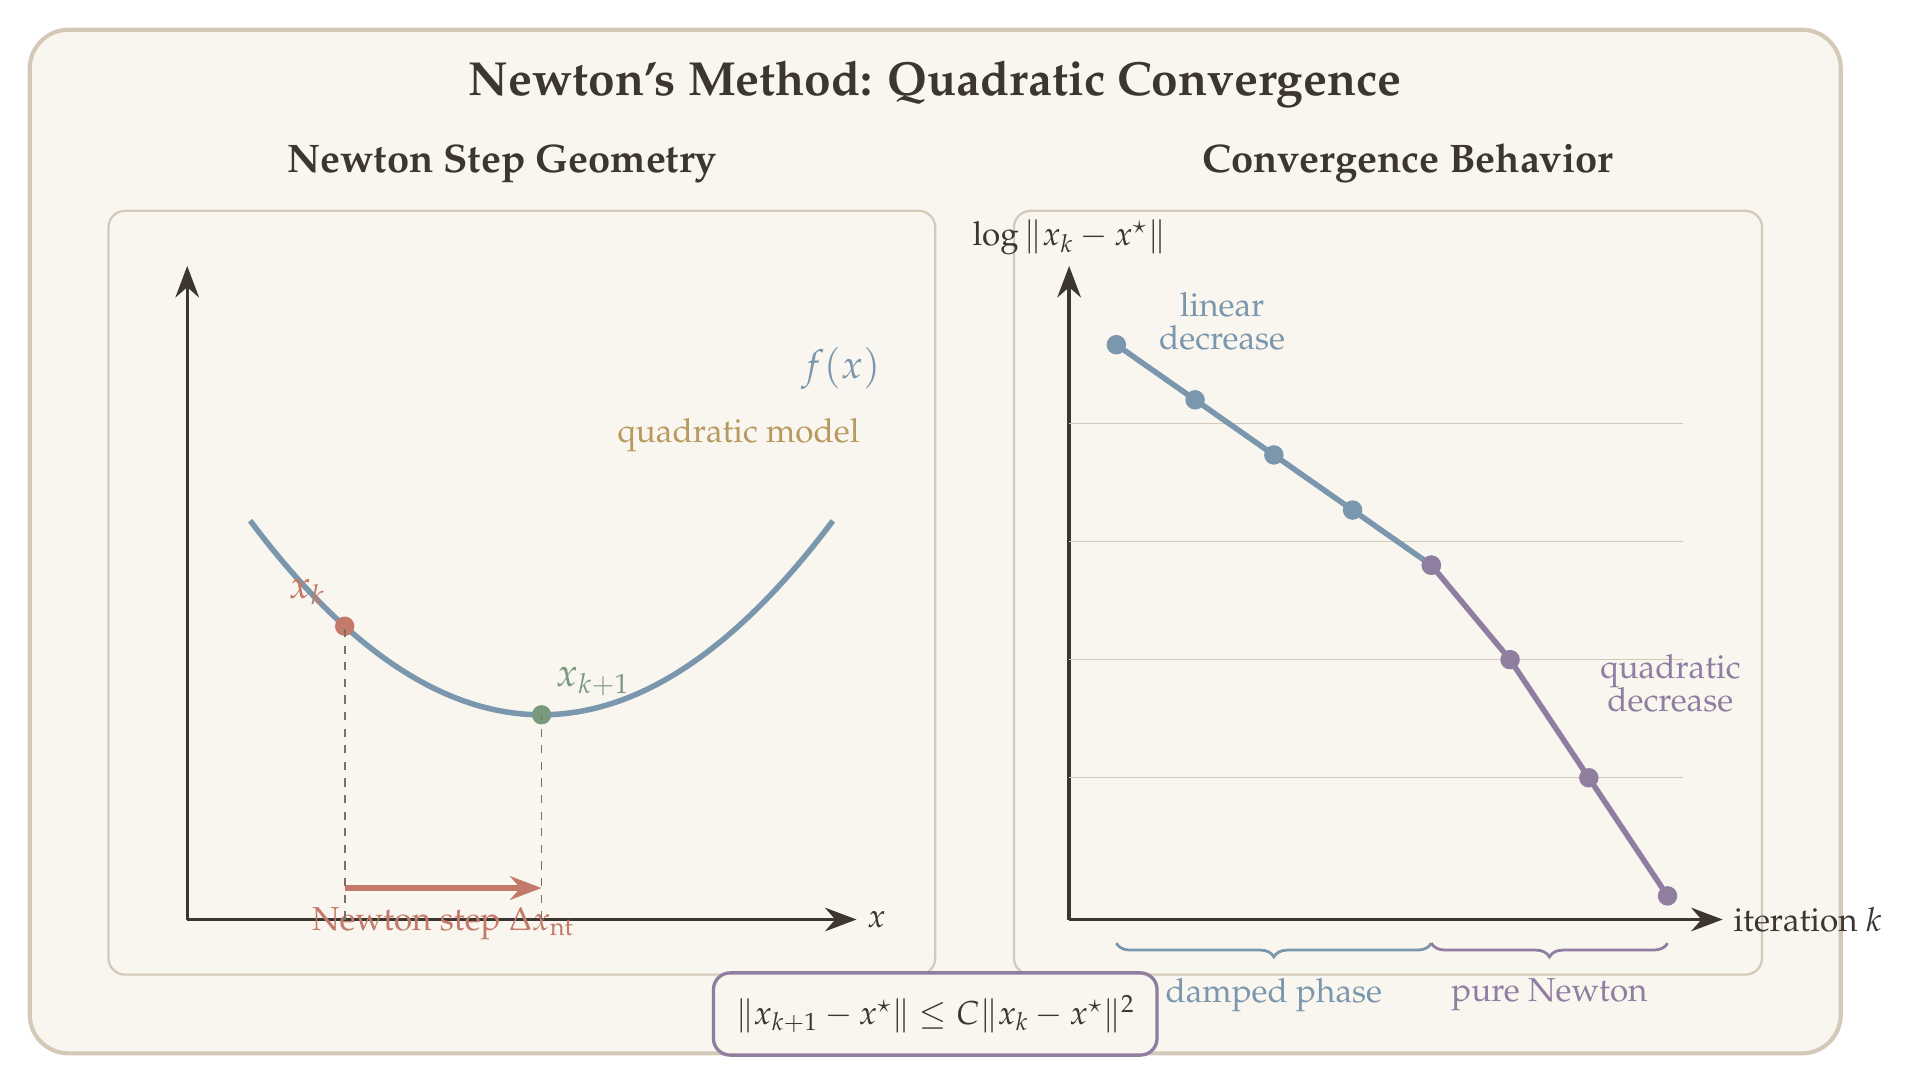
\begin{tikzpicture}[>={Stealth[length=4mm, width=3mm]}, line width=1.5pt]

% Background
\fill[cream, rounded corners=14pt] (-2,-3.5) rectangle (21,9.5);
\draw[border, line width=1.5pt, rounded corners=14pt] (-2,-3.5) rectangle (21,9.5);

% Title
\node[font=\LARGE\bfseries, text=dkbrown] at (9.5,8.8) {Newton's Method: Quadratic Convergence};

% =========== LEFT PANEL: Newton Step ===========
\node[font=\Large\bfseries, text=dkbrown] at (4,7.8) {Newton Step Geometry};

% Left panel box
\draw[border, line width=0.8pt, rounded corners=6pt] (-1,-2.5) rectangle (9.5,7.2);

% Axes
\draw[->, dkbrown, line width=1.2pt] (0,-1.8) -- (8.5,-1.8) node[right, font=\large, text=dkbrown] {$x$};
\draw[->, dkbrown, line width=1.2pt] (0,-1.8) -- (0,6.5) node[above, font=\large, text=dkbrown] {};

% Quadratic approximation (dashed)
\draw[rwgold, line width=1.5pt, dashed, smooth, samples=60, domain=0.8:8]
  plot (\x, {1.925 + (-0.9)*(\x-2) + 0.18*(\x-2)*(\x-2)});
\node[font=\large, text=rwgold, above] at (7,4.0) {quadratic model};

% Actual function
\draw[stblue, line width=2pt, smooth, samples=80, domain=0.8:8.2]
  plot (\x, {0.18*(\x-4.5)*(\x-4.5) + 0.8});
\node[font=\Large, text=stblue] at (8.3,5.2) {$f(x)$};

% x_k point
\fill[terracotta] (2, 1.925) circle (3.5pt);
\node[font=\Large, text=terracotta, above left] at (1.9, 2.05) {$x_k$};

% Newton step arrow
\draw[->, terracotta, line width=2pt] (2, -1.4) -- (4.5, -1.4);
\node[font=\large, text=terracotta, below] at (3.25, -1.5) {Newton step $\Delta x_{\mathrm{nt}}$};

% x_{k+1} point (minimum of quadratic = 4.5)
\fill[sage] (4.5, 0.8) circle (3.5pt);
\node[font=\Large, text=sage, above right] at (4.55, 0.9) {$x_{k+1}$};

% Dashed drop lines
\draw[wmgray, dashed, line width=0.6pt] (2, -1.8) -- (2, 1.925);
\draw[wmgray, dashed, line width=0.6pt] (4.5, -1.8) -- (4.5, 0.8);

% =========== RIGHT PANEL: Convergence Plot ===========
\node[font=\Large\bfseries, text=dkbrown] at (15.5,7.8) {Convergence Behavior};

% Right panel box
\draw[border, line width=0.8pt, rounded corners=6pt] (10.5,-2.5) rectangle (20,7.2);

% Axes
\draw[->, dkbrown, line width=1.2pt] (11.2,-1.8) -- (19.5,-1.8) node[right, font=\large, text=dkbrown] {iteration $k$};
\draw[->, dkbrown, line width=1.2pt] (11.2,-1.8) -- (11.2,6.5) node[above, font=\large, text=dkbrown] {$\log \|x_k - x^\star\|$};

% Grid lines
\foreach \y in {0,1.5,3,4.5} {
  \draw[border, line width=0.4pt] (11.2,\y) -- (19,\y);
}

% Damped phase: linear convergence (iterations 0-4)
\draw[stblue, line width=2pt, mark=*, mark size=2.5pt]
  plot coordinates {(11.8,5.5) (12.8,4.8) (13.8,4.1) (14.8,3.4) (15.8,2.7)};

% Pure Newton phase: quadratic convergence (iterations 4-7)
\draw[lavender, line width=2pt, mark=*, mark size=2.5pt]
  plot coordinates {(15.8,2.7) (16.8,1.5) (17.8,0.0) (18.8,-1.5)};

% Damped phase label
\draw[decorate, decoration={brace, amplitude=5pt, mirror}, stblue, line width=1pt]
  (11.8,-2.1) -- (15.8,-2.1);
\node[font=\large, text=stblue, below] at (13.8,-2.4) {damped phase};

% Pure Newton phase label
\draw[decorate, decoration={brace, amplitude=5pt, mirror}, lavender, line width=1pt]
  (15.8,-2.1) -- (18.8,-2.1);
\node[font=\large, text=lavender, below] at (17.3,-2.4) {pure Newton};

% Annotations
\node[font=\large, text=stblue, align=center, right] at (12.2,5.8) {linear\\[-2pt]decrease};
\node[font=\large, text=lavender, align=center, right] at (17.8,1.2) {quadratic\\[-2pt]decrease};

% Formula annotation
\node[fill=cream, draw=lavender, line width=1.2pt, rounded corners=6pt,
      font=\large, text=dkbrown, align=center, inner sep=8pt]
  at (9.5,-3.0) {$\|x_{k+1} - x^\star\| \le C\|x_k - x^\star\|^2$};

\end{tikzpicture}
\end{document}
